\documentclass[border=12pt,tikz]{standalone}
\usepackage{fontspec}
\setmainfont{Helvetica Neue}
\setsansfont{Helvetica Neue}
\setmonofont{Menlo}
\usepackage{tikz}
\usetikzlibrary{positioning, arrows.meta, fit, backgrounds, calc, decorations.pathreplacing}

\definecolor{keep}{HTML}{E3F2FD}
\definecolor{keepborder}{HTML}{2196F3}
\definecolor{change}{HTML}{FFF3E0}
\definecolor{changeborder}{HTML}{FF9800}
\definecolor{discard}{HTML}{FFEBEE}
\definecolor{discardborder}{HTML}{E53935}
\definecolor{gray50}{HTML}{9E9E9E}
\definecolor{accent}{HTML}{7B1FA2}

\begin{document}
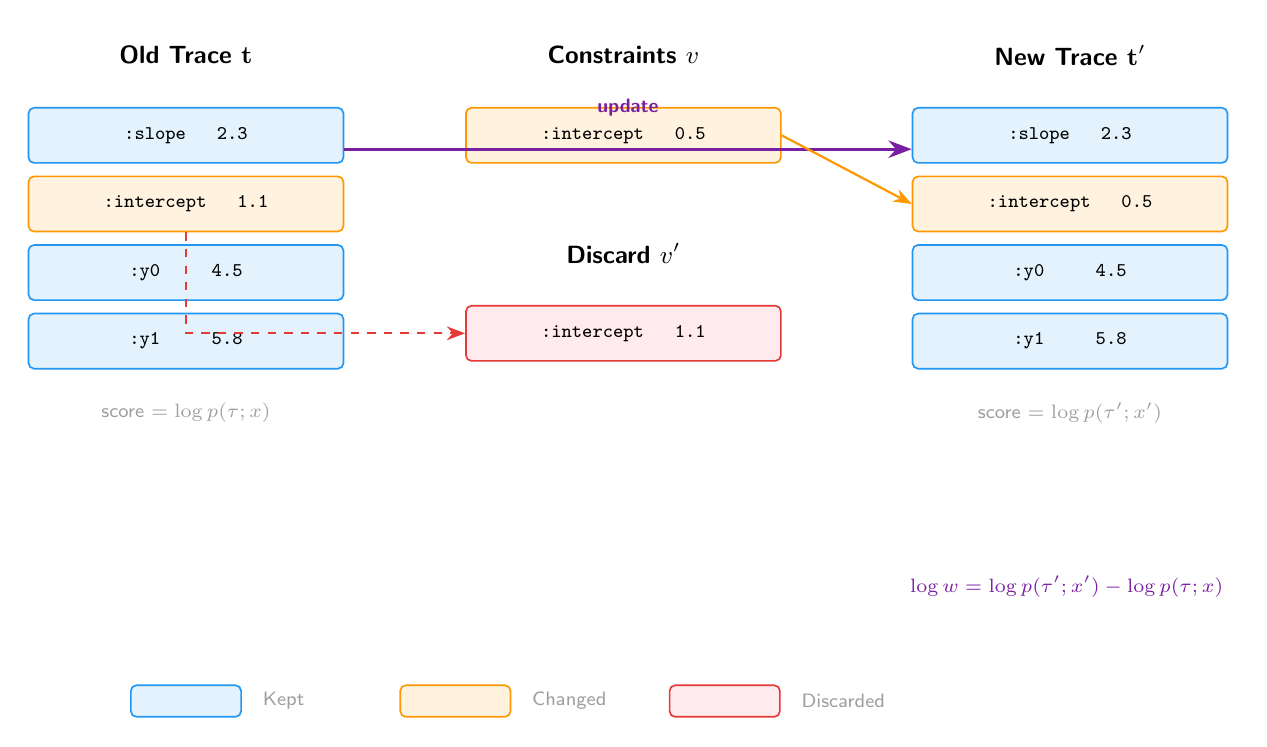
\begin{tikzpicture}[
    >=Stealth,
    node distance=0.6cm and 0.4cm,
    entry/.style={draw, rounded corners=2pt, minimum height=0.7cm, minimum width=4cm,
                  font=\ttfamily\scriptsize, line width=0.6pt, align=left},
    keepentry/.style={entry, fill=keep, draw=keepborder},
    changeentry/.style={entry, fill=change, draw=changeborder},
    discardentry/.style={entry, fill=discard, draw=discardborder},
    traceheader/.style={font=\sffamily\small\bfseries, minimum height=0.7cm},
    label/.style={font=\sffamily\scriptsize, color=gray50},
]

% === OLD TRACE (left) ===
\node[traceheader] (oldtitle) {Old Trace $\mathbf{t}$};
\node[keepentry, below=0.3cm of oldtitle] (old-slope) {:slope \quad 2.3};
\node[changeentry, below=0.15cm of old-slope] (old-inter) {:intercept \quad 1.1};
\node[keepentry, below=0.15cm of old-inter] (old-y0) {:y0 \quad\quad 4.5};
\node[keepentry, below=0.15cm of old-y0] (old-y1) {:y1 \quad\quad 5.8};

\node[label, below=0.3cm of old-y1] {score $= \log p(\boldsymbol{\tau}; x)$};

% === CONSTRAINTS (middle top) ===
\node[traceheader, right=3.5cm of oldtitle] (constitle) {Constraints $\boldsymbol{v}$};
\node[changeentry, below=0.3cm of constitle, minimum width=4cm] (con-inter) {:intercept \quad 0.5};

% === NEW TRACE (right) ===
\node[traceheader, right=3.5cm of constitle] (newtitle) {New Trace $\mathbf{t}'$};
\node[keepentry, below=0.3cm of newtitle] (new-slope) {:slope \quad 2.3};
\node[changeentry, below=0.15cm of new-slope] (new-inter) {:intercept \quad 0.5};
\node[keepentry, below=0.15cm of new-inter] (new-y0) {:y0 \quad\quad 4.5};
\node[keepentry, below=0.15cm of new-y0] (new-y1) {:y1 \quad\quad 5.8};

\node[label, below=0.3cm of new-y1] {score $= \log p(\boldsymbol{\tau}'; x')$};

% === DISCARD (below constraints) ===
\node[traceheader, below=1.8cm of constitle] (distitle) {Discard $\boldsymbol{v}'$};
\node[discardentry, below=0.3cm of distitle, minimum width=4cm] (dis-inter) {:intercept \quad 1.1};

% === ARROWS ===
% Old trace -> new trace
\draw[->, line width=1.2pt, color=accent] ([yshift=-5pt]old-slope.east) -- ([yshift=-5pt]new-slope.west)
    node[midway, above, font=\sffamily\scriptsize\bfseries, color=accent, yshift=8pt] {update};

% Constraints -> new trace
\draw[->, line width=0.8pt, color=changeborder] (con-inter.east) -- (new-inter.west);

% Old value -> discard
\draw[->, line width=0.8pt, color=discardborder, dashed] (old-inter.south) |- (dis-inter.west);

% Weight annotation
\node[font=\sffamily\scriptsize, color=accent, below=2.5cm of new-y1, align=center] {
  $\log w = \log p(\boldsymbol{\tau}'; x') - \log p(\boldsymbol{\tau}; x)$
};

% Legend
\node[keepentry, minimum width=1.4cm, minimum height=0.4cm, below=4cm of old-y1] (legkeep) {};
\node[label, right=4pt of legkeep] {Kept};
\node[changeentry, minimum width=1.4cm, minimum height=0.4cm, right=2cm of legkeep] (legchange) {};
\node[label, right=4pt of legchange] {Changed};
\node[discardentry, minimum width=1.4cm, minimum height=0.4cm, right=2cm of legchange] (legdiscard) {};
\node[label, right=4pt of legdiscard] {Discarded};

\end{tikzpicture}
\end{document}
